\documentclass[runningheads]{llncs}

\usepackage{natbib}

\usepackage[T1]{fontenc}

\usepackage{amsfonts}

\usepackage{amsmath}

\usepackage{graphicx}

\usepackage{svg}

\usepackage{acronym}

\usepackage{hyperref}

\usepackage{subfig}



\newcommand{\topic}{Approaches for finding sample pairs in contrastive learning}
\newcommand{\authorA}{Klara M. Gutekunst}

% If you use the hyperref package, please uncomment the following two lines
% to display URLs in blue roman font according to Springer's eBook style:
%\usepackage{color}
%\renewcommand\UrlFont{\color{blue}\rmfamily}
%\urlstyle{rm}
%
\begin{document}

%
\title{\topic}
%
\titlerunning{\topic}

\author{\authorA}
%
\authorrunning{\authorA}

\institute{University of Kassel, Germany\\
\email{klara.gutekunst@student.uni-kassel.de}}
%
\maketitle         
%
% include: speed bonus, no reloads, but no nesting, forces page break after and before input
\begin{abstract}
    %The abstract should briefly summarize the contents of the paper in
    %150--250 words.
    % unsupervised learning
    Since labelled data is often scarce and expensive to obtain, 
    unsupervised learning has emerged as a powerful paradigm for training models without reliance on labelled data. 
    % SSL
    Within this domain, \acl{ssl} has gained significant attention, leveraging unlabelled data to generate labels.
    % CL
    A core concept within \acl{ssl} is \acl{cl}, which focuses on learning data representations by contrasting positive and negative sample pairs. 
    % representation learning
    The key idea is to encourage the model to map positive samples closer together in the representation space 
    while pushing negative samples farther apart.
    % hard positive/ negative pairs
    The selection of positive and negative pairs is of particular importance, 
    as challenging pairs present valuable learning opportunities for the model.
    % motivation
    A significant advantage of \acl{cl} in representation learning is its ability to capture the underlying structure of the data, 
    leading to the development of more robust and generalizable models.
    % this paper
    This review paper offers a comprehensive examination of various \acl{cl} approaches, 
    focusing on their foundational principles and the methods employed for pair selection, 
    while also providing a critical analysis of these techniques.
    
    \keywords{\acl{cl}  \and \acl{ssl} \and Hard sample mining.}
\end{abstract}

\section{Introduction}\label{sec:introduction}

\acf{ssl} is an unsupervised learning technique that allows training models on data without any labels.
The idea is to generate labels from the unlabelled training data contemplating a pre-text task.

% SSL
\acf{ssl} is an unsupervised learning technique that allows training models on data without any labels.
This is achieved through the use of pre-text tasks designed to create labels from the unlabelled dataset.
% pre-text task
Researchers usually select self-supervised pre-text tasks such that 
the labels can be generated without human annotations \citet{PIC_2020}.
% instance recognition
One such pre-text task, instance discrimination, treats each instance in the dataset as a distinct class.
% positive and negative samples
In a scenario where a dataset consists of multiple inherent (unlabelled) classes, 
instances from the same class are considered positive pairs, 
while instances from different classes are treated as negative pairs.
% goal
Consequently, the model learns to differentiate between instances and 
develops robustness to (image) transformations
\citet{PIC_2020,swav_2020,local_aggr_2019,grape_2024,CL_temp_2021}.

In order to explain why the proximity of generated samples to the anchor $x$ is relevant to the efficiency during training, 
one can consider a simple example in Euclidean space.
Imagine images as input to a \ac{nn}, which projects them onto $f_{\theta}(x) \in \mathbb{R}^d$, 
where $\theta$ are the parameters of the \ac{nn}.
The effect of the distance between the anchor $x$ and the positive $x^+$ (negative $x^-$) 
sample on the loss is visualized in \autoref{fig:hard_easy_samples_dist_effect_loss}.
Since difficult samples hold more (gradient) information, they have a higher loss value.
Hence, similar negative pairs ($x$, $x^-$) are considered hard \citet{robinson_contrastive_2021}, 
while distant positive pairs ($x$, $x^+$) are considered hard.

% \begin{figure}[h] % h = here, t = top, b = bottom, p = page of floats
%     \centering
%     \includesvg[width=300pt]{images/Hard_easy_samples_dist_effect_loss}
%     \caption{The impact of the distance between a generated sample and its anchor on the loss function.
%     Hard samples convey more (gradient) information than easy samples and thus, have a higher loss value.
%     While distant positive pairs are considered hard, for negative samples, small proximity ones are considered hard.}
%     \label{fig:hard_easy_samples_dist_effect_loss}
% \end{figure}

\begin{figure}[h] % h = here, t = top, b = bottom, p = page of floats
    \centering
    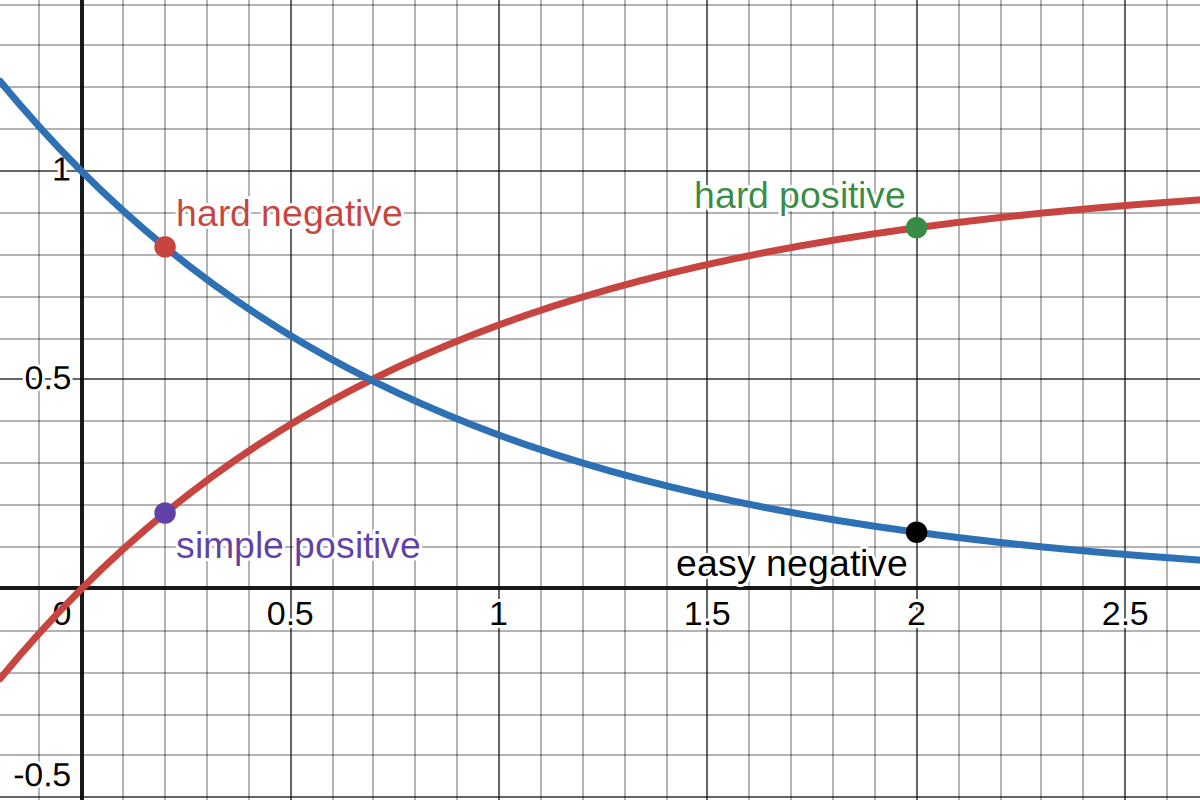
\includegraphics[width=280pt]{images/Hard_easy_samples_dist_effect_loss_desmos.png}
    \caption{The impact of the distance between a generated sample and its anchor on the loss function.
    The red curve represents the loss function for positive samples, 
    whereas the blue curve denotes negative samples.
    Hard samples convey more (gradient) information than easy samples and thus, have a higher loss value.
    While distant positive pairs are considered hard, for negative samples, small proximity ones are considered hard.}
    \label{fig:hard_easy_samples_dist_effect_loss}
\end{figure}

% main part



The selection of positive pairs ($x$, $x^+$) is subject to multiple papers, 
which propose different strategies.
In the case of unsupervised learning, generally, 
the positive sample $x^+$ is generated by applying a transformation to the anchor $x$.
Popular image augmentation techniques include random cropping, color jittering, Gaussian blur,
rotation and scaling \citet{ho_contrastive_2020,robinson_contrastive_2021,curricular_weighting_2024}.
Graph augmentations involve adding or removing edges and nodes, 
whereas in words or sentences are added or masked in the context of natural language processing 
\citet{curricular_weighting_2024}.

% PU learning
Another approach is to use so-called \ac{pu} learning, where learning is carried out 
on a set of positive and a set of unlabeled samples \citet{chuang_debiased_2020}.

% unsupervised learning
Simple selection techniques of negative samples include uniform sampling from the dataset or batch.
However, this approach is prone to two issues \citet{robinson_contrastive_2021,mining_potential_2024}:
\begin{enumerate}
    \item Selected samples are not necessarily hard negatives since the approach does not consider the embedding space proximity.
    \item Selected samples might actually belong to the same class as the anchor and thus, can be denoted \ac{fn}.
\end{enumerate}

% oracle learning
Some approaches use a so-called class oracle to boost the performance of the model.
If \acp{fn} \cite{grape_2024,curricular_weighting_2024,progcl_2022}, i.e. samples considered negative that belong to the latent class of the anchor,
 are sampled during hard negative mining samples of the same class are pushed further apart in the embedding space. 
To avoid performance deterioration, this approach removes the \acp{fn} from the set of negative samples and thus, 
increases the performance of the model \citet{mochi_2020}.

\section{Related Work}\label{sec:related_work}

% sampling from distributions
Naturally, when using descriptive statistics to describe data, (empirical estimated) distributions play a crucial role.
Some researchers obtain their positive and negative samples from distributions.
Unfortunately, since \ac{cl} is a form of unsupervised learning, 
the true data distribution of the different classes is often not available.
Therefore, some scientists formulate assumptions or simplify the problem.
Possible assumptions include that the data distribution is uniform,
or approximating the positive sample distribution by sampling from a set of transformations 
or using the overall data distribution as a proxy for the negative sample distribution \citet{chuang_debiased_2020,robinson_contrastive_2021}.
In other cases, the class distributions are approximated using \acp{bmm} \citet{progcl_2022}.

Given the assumption that the data distribution sufficiently well approximated, 
it is possible to consider probabilities of samples being \acp{fn} during the selection process of samples.
Needless to say, the goal is to avoid sampling \acp{fn} as negative samples.
To this end, scientists have proposed different strategies, which mostly boil down to 
incorporating the possibility of a potential negative sample being a \ac{fn} or \ac{tn} 
\citet{chuang_debiased_2020,robinson_contrastive_2021,progcl_2022}.


% augmentation strategies
Irrespective of its usage in the context of estimation of distributions, 
data augmentation is a common technique to create positive samples.
Often, an augmentation strategy is randomly sampled from a set of possible augmentations.
The motivation behind this is to increase the diversity of the positive samples 
in order to drive the model to learn features invariant to translations 
\citet{PIC_2020,swav_2020,local_aggr_2019,grape_2024,CL_temp_2021}.


% clustering/ distance
Since \ac{cl} objectives are often formulated in terms of distances or similarities between pairs of samples, 
the idea of using clustering techniques is a natural choice.
Intuitively, clusters of similar samples should be considered as positive samples and thus,
should be encoded close to each other.
Conversely, samples from different clusters should be encoded far apart.

Multiple methods have been proposed to generate samples via clustering.
Some ideas focus on high intra-cluster similarities to improve the alignment of the embeddings \citet{DRC_2020}.
Other ideas define different neighbour regions to condense representation within an inner radius 
while repelling samples from an outer radius \citet{local_aggr_2019}.
Another approach is to consider both Euclidean distance and semantic similarity to generate hard samples \citet{mining_manifolds_2018}.
Moreover, the \ac{pcl} technique defines positive samples as cluster centroids 
from one of the multiple clusterings for different numbers of clusters 
to encode the hierarchical structure of the data \citet{PCL_2021}.


% memory bank
Another prominent concept is the usage of memory banks to store embeddings of the data.
\citeauthor{mochi_2020} fill these memory banks with embeddings of negative samples 
and propose two approaches for generating new hard negatives: 
Two of the most difficult samples currently stored in the memory bank are randomly selected and mixed.
The second approach is to use only one of the existing negative samples and 
mix it with the anchor to create a new sample.

\citet{progcl_2022} propose a method that extends the idea of \citet{mochi_2020} by weighting randomly selected negative samples 
with their relative similarity to the anchor when mixing them to create more difficult negative samples.

It is also possible to use the memory bank to store the embeddings of the positive samples.
Similarly, either randomly chosen samples can be used individually or 
the samples can be weighted by their hardness during loss calculation \citet{mining_potential_2024}.


% other work
% EM-algorithm
Multiple approaches, including \ac{drc}, \ac{pcl} and \progcl{}, use the \ac{em} algorithm 
to reduce computational costs or to find solutions via approximations.
Both \ac{drc} \citet{DRC_2020} and \progcl{} \citet{PCL_2021} are clustering-based methods 
while \progcl{} \citet{progcl_2022} is a distribution-based method.

% temperature
Since most approaches use a temperature parameter to control the hardness of the negative samples, 
\citet{CL_temp_2021} and \citet{grape_2024} investigate the impact of the temperature on the performance of the model.
They find that the \ac{cl} loss function optimizes hard samples by penalizing them according to their hardness.
If the temperature is small, only the closest points are penalized and others are not.
This can result in a uniformly distributed embedding space.

% curriculum learning
\citet{curricular_weighting_2024} propose a curriculum learning approach to generate hard negative samples.
They outline why curriculum learning is beneficial for \ac{cl} and how it can be implemented.

% data scheduling
% \citet{PIC_2020} propose a method to schedule the data for training 
% to reduce the periods within which a sample is not considered for training.

\section{Sampling techniques}\label{sec:sampling_techniques}

Since positive pairs ($x$, $x^+$) are considered to originate from the same class, we denote $\rho(c), c \in \mathcal{C}$ as the distribution over the latent classes.
Moreover, let $h: \mathcal{X} \rightarrow \mathcal{C}$ be the ground truth assigning class labels $c \in \mathcal{C}$ to inputs $x \in \mathcal{X}$.
Hence, $x \sim x'$ if $h(x) = h(x')$ \citet{robinson_contrastive_2021,chuang_debiased_2020}.
Assuming that $\rho(c)$ is uniformly distributed, and that $x^- \sim q = p$ where the anchor $x$ 
is drawn from the data distribution $p$.

\subsection{Robinson's Hard Negatives}\label{subsec:robinson_hard_negatives}

\citet{robinson_contrastive_2021} 
propose a novel approach to sample hard negatives from $q \neq p$.
This method balances both the risk of sampling \ac{fn} and the degree of hardness of the samples obtained.
Moreover, via the concentration parameter $\beta$, the user can decide how hard the negatives should be and thus, how likely they have the same target as the anchor.
Large values of $\beta$ lead to sampling very hard negative samples.
The authors of \citet{robinson_contrastive_2021} propose negative samples from $q^-_{\beta}(x^-)$, 
which enforces $x$, $x^-$ having different classes by conditioning on dissimilar classes.
By computing a scalar product of both representations $f(x)$, $f(x^-)$ in \eqref{eq:q_beta}, 
they encourage similar represented samples.
Unfortunately, it is unclear how to sample from $q^-_{\beta}(x^-)$ and thus, 
the authors propose a way to rewrite the equation to facilitate sampling.

\begin{align} 
    q^-_{\beta}(x^-) = q_\beta(x^-|h(x) \neq h(x^-)) \propto \exp(\beta f(x)^\text{T}f(x^-))\cdot p(x^-) 
\label{eq:q_beta}
\end{align} 


Since sampling could both yield \ac{fn} and \ac{tn}, it is possible to rewrite \eqref{eq:q_beta_minus} 
displaying both cases in \eqref{eq:fn_tn}.
The first term corresponds to the probability of sampling \ac{tn}, i.e. $h(x) \neq h(x^-)$,
 while the second term corresponds to the probability of sampling \ac{fn} with $x \sim x^-$.

\begin{align}
    q_\beta(x^-) &= \rho(c)q^{-}_\beta(x^-) + (1-\rho(c))q^{+}_\beta(x^-)
    \label{eq:fn_tn}
\end{align}

The distribution $q^{+}_\beta(x^-)$ can described in more detail.
Given that $x$ and $x^-$ are from the same class, 
the probability of sampling $x^-$ is proportional to the exponential of the scalar product of the 
representations of $x$ and $x^-$ as described in \eqref{eq:q_beta_plus}.

\begin{align}
    q^{+}_\beta(x^-) &= q_\beta(x^-|h(x) = h(x^-)) &\propto \exp(\beta f(x)^\text{T}f(x^-))\cdot p^+(x^-) 
    \label{eq:q_beta_plus}
\end{align}

Finally, we can rewrite \eqref{eq:fn_tn} to obtain the desired distribution $q^-_{\beta}(x^-)$ as shown in \eqref{eq:q_beta_minus}.
This version of the distribution allows for sampling from $q^-_{\beta}(x^-)$, since we can sample from $q_\beta(x^-) \approx p$ 
and we can approximate $q^{+}_\beta(x^-)$ by sampling from a set of transformations.    % rejection sampling & Monte Carlo sampling

\begin{align}
    q^{-}_\beta(x^-) &= \frac{(q_\beta(x^-)-(1-\rho(c))q^{+}_\beta(x^-))}{\rho(c)} 
    \label{eq:q_beta_minus}
\end{align}



% \begin{align*}
%     q^{-}_\beta(x^-) &=  q_\beta(x^-|h(x) \neq h(x^-)) 
% &\propto \exp(\beta f(x)^\text{T}f(x^-))\cdot p(x^-) 
% \\&= \rho(c)q^{-}_\beta(x^-) + (1-\rho(c))q^{+}_\beta(x^-)
% \\&= \rho(c)\frac{(q_\beta(x^-)-(1-\rho(c))q^{+}_\beta(x^-))}{\rho(c)} + (1-\rho(c))q_\beta(x^-|h(x) = h(x^-)) &\propto \rho(c)q^{-}_\beta(x^-) + \exp(\beta f(x)^\text{T}f(x^-))\cdot p^+(x^-) 
% \end{align*}

\subsection{Adversarial Examples}\label{subsec:adversarial_examples}

\cite{ho_contrastive_2020}

\subsection{Debiased Contrastive Learning}\label{subsec:debiasing_cl}

\subsection{\acl{drc}}\label{subsec:drc}

\citeauthor{DRC_2020} propose a method called \ac{drc} 
that faces issues of high intra-class diversities 
due to structural shortcomings in existing deep clustering methods.
They claim that existing methods enforce the representations of samples 
and their augmentations to be assigned to the same cluster,
due to the usage of the maximum sensitivity of the softmax function used during cluster assignment.

\ac{drc} aims to address this issue by considering both the \ac{af} and the \ac{ap} during clustering.
Even though the \ac{ap} can be similar for different samples, their \ac{af} can be different 
as illustrated in \autoref{fig:drc_af_ap}.

\begin{figure}[h] % h = here, t = top, b = bottom, p = page of floats
    \centering
    \includegraphics[width=300pt]{images/DRC_af_ap.png}
    \caption{Similar \ac{ap} values for different samples, but different \ac{af} values from \citet{DRC_2020}.
    Cluster assignment based on only \ac{ap} values can result in high intra-cluster diversities.}
    \label{fig:drc_af_ap}
\end{figure}

\subsubsection{\acl{la}}\label{subsec:local_aggregation}

% s. unten: Hyperparameter prob- woher? k, H ist getestet, zumindest das Verhältnis, aber lambda wird aus anderer Arbeit übernommen -> keine Hyperparameter Suche

\citet{local_aggr_2019} optimizes a low-dimensional feature space mapping by 
iteratively identifying close neighbours and updating the embedding function.
This soft clustering technique is called \ac{la}.

At each step during training of the embedding function $f_\theta: \mathcal{X} \rightarrow \mathcal{Z}$, 
two sets of neighbours are identified for each datapoint's embedding $z_i$ 
which are illustrated in \autoref{fig:la_bi_ci}.
The first set $C_i$ contains $z_i$'s close neighbours in the feature space, while
the second set $B_i$ contains $z_i$'s background neighbours.
$B_i$ is used as a means to judge distance and similarity, 
while $C_i$'s members should be embedded closer to $z_i$.
In other words, $C_i$ can be considered the set of positive samples while 
$B_i$ denotes the set of negative samples.
The level of \ac{la} $L(C_i,B_i | \theta, x_i)$ 
characterizes the relative level of closeness within $C_i$ compared to $B_i$.
$L(C_i,B_i | \theta, x_i)$ should be maximized.

The set $B_i$ consists of the $k$ nearest neighbours of $z_i$ in terms of cosine distance 
in the feature space.
$k$ is a hyperparameter and \citet{local_aggr_2019} set $k=4096$.
In order to construct $C_i$, 
first $H$ $k$-means clusterings are performed with sligthly different conditions.
Then, all of $z_i$'s clusters are united to form $C_i$.
$H$ and $k$ are hyperparameters.
\citet{local_aggr_2019} find that more clusterings, i.e. higher $H$, leads to isotropic clusters since outliers which arise from random processes are averaged out.
Moreover, if $H$ is too high compared to the number of clusters $k$, the performance decreases.
They state that $H=3, k=10000$ and $H=10, k=30000$ are better values than $H=10, k=10000$ 
in terms of ResNet-18 nearest neighbour validation performance.

Finally, the level of \ac{la} $L(C_i,B_i | \theta, x_i)$ is defined as the negative log-likelihood 
of the feature space representation $z_i$ of $x_i$ being in $C_i$ given $B_i$, 
i.e., being recognized as a close neighbour given being recognized as a background neighbour.
The loss to minimize is $\mathcal{L} = L(C_i,B_i | \theta, x_i) + \lambda \left\| \theta \right\|^2$.
\citet{local_aggr_2019} choose to rely on hyperparameter settings from another work rather than conducting a hyperparameter search.

\begin{figure}[h] % h = here, t = top, b = bottom, p = page of floats
    \centering
    \includegraphics[width=360pt]{images/la_neighbourhoods.png}
    \caption{Illustration from \citet{local_aggr_2019}.
    A \ac{cnn} produces the feature space embedding $z_i = f_\theta(x_i)$.
    The embeddings are displayed as points in the feature space.
    The red point is the anchor $z_i$, 
    whereas blue points are close neighbours $C_i$ and
    black points are background neighbours $B_i$.
    The arrows denote influences between the neighbours.}
    \label{fig:la_bi_ci}
\end{figure}

% end

% ---- Bibliography ----

% \bibliographystyle{splncs04}
\bibliographystyle{unsrtnat}
\bibliography{references}



\begin{acronym}

    \acro{nn}[NN]{Neural Network}

\end{acronym}

\end{document}
